\title[Phát hiện bất thường theo ngữ cảnh có thể giải thích]{Phát hiện bất thường theo ngữ cảnh có thể giải thích bằng cách sử dụng Rừng hồi quy phân vị \footnote{Bản thảo được chấp nhận bởi tạp chí \textit{Khai thác dữ liệu và khám phá kiến ​​thức} để xuất bản (2023 tháng 6). Đây là phiên bản in sẵn.}}


\author*{\fnm{Zhong} \sur{Li}}\email{z.li@liacs.leidenuniv.nl}

\author{\fnm{Matthijs} \sur{van Leeuwen}}\email{
m.van.leeuwen@liacs.leidenuniv.nl}

\affil{\orgdiv{Viện khoa học máy tính tiên tiến Leiden (LIACS)}, \orgname{Đại học Leiden}, \country{Hà Lan}}



\abstract{Các phương pháp phát hiện bất thường truyền thống nhằm mục đích xác định các đối tượng khác với hầu hết các đối tượng khác bằng cách xử lý tất cả các đặc điểm như nhau. Ngược lại, các phương pháp phát hiện sự bất thường theo ngữ cảnh nhằm mục đích phát hiện các đối tượng đi chệch khỏi các đối tượng khác trong một \emph{bối cảnh} gồm các đối tượng tương tự bằng cách chia các đặc điểm thành các đặc trưng ngữ cảnh và các đặc trưng hành vi. Trong bài viết này, chúng tôi phát triển mối liên hệ giữa các phương pháp phát hiện bất thường truyền thống dựa trên sự phụ thuộc và các phương pháp phát hiện bất thường theo ngữ cảnh. Dựa trên những hiểu biết sâu sắc thu được, chúng tôi đề xuất một cách tiếp cận mới để phát hiện sự bất thường theo ngữ cảnh vốn có thể giải thích được bằng cách sử dụng Rừng hồi quy phân vị để mô hình hóa sự phụ thuộc giữa các tính năng. Các thử nghiệm mở rộng trên nhiều tập dữ liệu tổng hợp và thế giới thực khác nhau chứng minh rằng phương pháp của chúng tôi vượt trội hơn các phương pháp phát hiện bất thường hiện đại trong việc xác định các điểm bất thường theo ngữ cảnh về độ chính xác và khả năng giải thích.}

\keywords{Phát hiện bất thường, Giải thích bất thường, Phát hiện ngoại lệ, Phát hiện bất thường theo ngữ cảnh, Rừng hồi quy phân vị }



\maketitle

\section{Giới thiệu}
\label{sec:introduction}

Theo định nghĩa nổi tiếng của \cite{hawkins1980identification}, một dị thường\footnote{Do thực tế là ``ngoại lệ' thường được sử dụng như một từ đồng nghĩa với `` dị thường "trong tài liệu phát hiện bất thường, nên chúng tôi sẽ sử dụng chúng thay thế cho nhau trong bài viết này.} là một đối tượng có sự khác biệt đáng kể so với hầu hết các đối tượng còn lại. \cite{chandola2009anomaly} chia các dị thường thành ba loại: dị thường điểm (một đối tượng được coi là dị thường khi so sánh với các đối tượng còn lại), bất thường theo ngữ cảnh (một đối tượng là bất thường trong một ngữ cảnh cụ thể) và dị thường tập thể (một tập hợp các đối tượng là bất thường đối với toàn bộ tập dữ liệu). Việc phân tích các điểm bất thường có nhiều ứng dụng, chẳng hạn như trong bảo mật mạng \citep{ahmed2016survey1}, tin sinh học \citep{spinosa2005support}, phát hiện gian lận \citep{ahmed2016survey2} cũng như phát hiện và cách ly lỗi \citep{hwang2009survey}.Phân tích sự bất thường bao gồm hai nhiệm vụ quan trọng như nhau: phát hiện sự bất thường và giải thích sự bất thường. Rất nhiều phương pháp dựa trên học máy “nông”, tức là không dựa trên học sâu, đã được đề xuất để phát hiện các điểm bất thường \citep{chandola2009anomaly}. Gần đây, nhiều phương pháp phát hiện bất thường dựa trên deep learning cũng đã được phát triển \citep{pang2021deep}.
Tuy nhiên, các phương pháp phát hiện điểm bất thường dựa trên deep learning nổi tiếng là không thể diễn giải được, theo nghĩa là nhìn chung cả bản thân mô hình đều không minh bạch và kết quả là điểm bất thường rất khó diễn giải nếu không sử dụng trình giải thích hậu kỳ. Trong bài viết này, đặc biệt là vấn đề sau mà chúng tôi cho là có vấn đề, vì các giải thích hậu nghiệm thường không chỉ dựa vào mô hình mà còn dựa vào người giải thích cụ thể được sử dụng. Ngoài ra, các phương pháp học sâu thường yêu cầu lượng lớn dữ liệu và việc đào tạo các mô hình là một quá trình tốn thời gian. Tuy nhiên, trong nhiều ứng dụng trong thế giới thực, khả năng diễn giải 'bản địa' (tức là không có trình giải thích hậu nghiệm) có thể được yêu cầu và có thể có sẵn dữ liệu và/hoặc thời gian tính toán hạn chế. Vì những lý do này, trong bài viết này, chúng tôi hạn chế tập trung vào các phương pháp dựa trên học máy “nông cạn”. Để phù hợp với lựa chọn này, chúng tôi tập trung vào các cài đặt trong đó lượng dữ liệu nhỏ hơn mức yêu cầu thông thường để tìm hiểu các mô hình sâu chính xác. Hầu hết các phương pháp nông hiện có chỉ xem xét phát hiện điểm bất thường, phần lớn bỏ qua phát hiện bất thường theo ngữ cảnh. Hơn nữa, lời giải thích về sự bất thường đã nhận được rất ít sự chú ý. Trong bài viết này, chúng tôi giải quyết cả vấn đề phát hiện sự bất thường theo ngữ cảnh và vấn đề giải thích sự bất thường, đối với dữ liệu dạng bảng có kích thước nhỏ đến vừa phải có các đặc điểm phân loại và/hoặc định lượng.

\begin{figure}[tb]
\centering
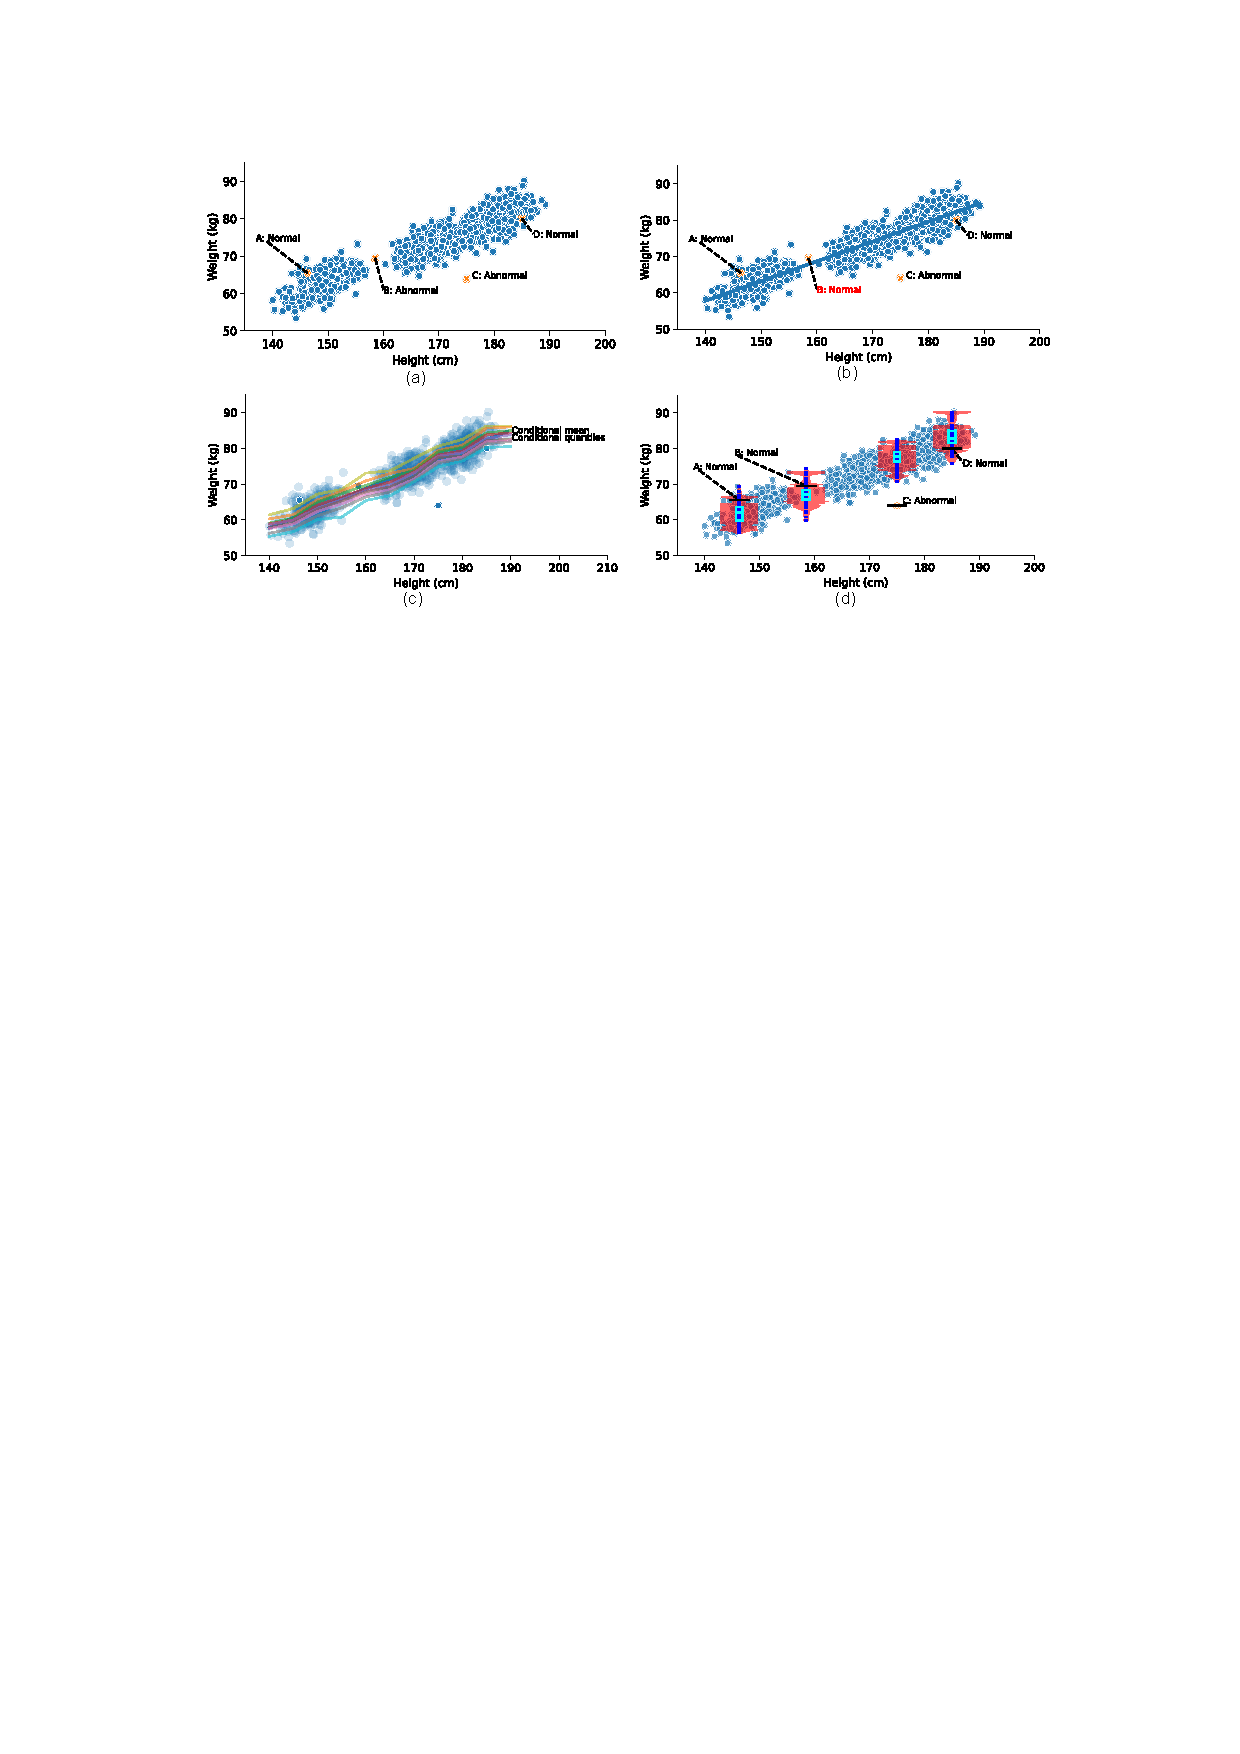
\includegraphics[width=12cm]{images/Pic_introduction.pdf}
\caption{Các loại phát hiện bất thường khác nhau. (a) Các phương pháp dựa trên khoảng cách và mật độ đều coi đối tượng B là bất thường, vì nó ở xa các đối tượng khác và ở vùng mật độ thấp. (b) Các phương pháp dựa trên sự phụ thuộc mô hình hóa mối quan hệ giữa chiều cao và cân nặng và do đó coi đối tượng B là bình thường. (c) Các phân vị có điều kiện cung cấp nhiều thông tin về phân bố có điều kiện hơn là chỉ giá trị trung bình và (d) có thể được sử dụng để trực quan hóa --- sử dụng biểu đồ beanplot (hoặc nói đúng hơn là một biến thể của biểu đồ beanplot kết hợp với biểu đồ hộp, xem Phần \ref{qcad:ae} để biết chi tiết) --- tại sao một đối tượng nhất định được coi là (ab)bình thường.}\label{fig:intro}
\end{figure}Các máy phát hiện bất thường nông thường được phân loại thành các phương pháp tiếp cận dựa trên khoảng cách, dựa trên mật độ và dựa trên phân phối \citep{wang2019progress}. Các phương pháp dựa trên khoảng cách và mật độ sử dụng kiến ​​thức về khoảng cách không gian của các đối tượng để xác định điểm bất thường, trong khi các phương pháp dựa trên phân phối sử dụng kiến ​​thức về phân bố dữ liệu để phát hiện điểm bất thường. Các phương pháp này hoạt động theo giả định rằng \textit{các đối tượng có khoảng cách lớn hoặc mật độ khác với các lân cận trong không gian của chúng là dị thường} hoặc \textit{các đối tượng có giá trị hiếm theo phân bố biên hoặc phân bố chung của các đặc điểm tương ứng là dị thường}. Tuy nhiên, việc sử dụng một trong hai giả định này có thể dẫn đến kết quả dương tính giả. Ví dụ: như trong Hình~\ref{fig:intro}(a), các phương pháp này sẽ xác định nhầm đối tượng B là vật thể dị thường nếu mục đích là phát hiện những người thừa cân hoặc thiếu cân.

Vì điều này thường không mong muốn nên chúng tôi muốn xác định và phát hiện các điểm bất thường từ một góc độ khác, nghĩa là chúng tôi giả định rằng \textit{các đối tượng vi phạm sự phụ thuộc, tức là mối quan hệ giữa các tính năng, là bất thường}. Đây là ý tưởng đằng sau tính năng phát hiện bất thường dựa trên phụ thuộc \citep{lu2020dependency}, ý tưởng này không mới nhưng nhận được sự chú ý hạn chế so với các loại dị thường khác. Nó tận dụng cấu trúc và thuộc tính nội tại của dữ liệu để tìm ra những điểm bất thường có khả năng phù hợp hơn. Ví dụ: Hình \ref{fig:intro}(b) cho thấy phương pháp này sẽ xác định đối tượng B là bình thường bằng cách mô hình hóa sự phụ thuộc giữa chiều cao và cân nặng.

Các kỹ thuật phát hiện điểm bất thường truyền thống --- bao gồm các phương pháp dựa trên khoảng cách, mật độ và sự phụ thuộc --- xử lý tất cả các đặc điểm như nhau khi xác định điểm bất thường. Tuy nhiên, trong các lĩnh vực như chăm sóc sức khỏe, mạng cảm biến và bảo vệ môi trường, một số tính năng không bao giờ được sử dụng trực tiếp để định lượng sự bất thường. Ví dụ, hệ thống phát hiện cháy rừng không nên coi các giá trị “sai lệch” của vĩ độ, kinh độ, ngày và giờ là dấu hiệu của sự bất thường. Tuy nhiên, chúng ta không nên đơn giản loại bỏ những tính năng này vì chúng có thể chứa thông tin liên quan. Ví dụ: nhiệt độ 'bình thường' có thể cao hơn ở một số vùng nhất định so với các vùng khác. Điều này thúc đẩy chúng tôi điều tra việc \emph{phát hiện bất thường theo ngữ cảnh}, vốn có thể có thể tính đến các tính năng bổ sung như vậy.

Tính năng phát hiện sự bất thường theo ngữ cảnh giả định rằng \textit{một đối tượng là bất thường nếu nó đi chệch hướng mạnh so với các đối tượng trong `ngữ cảnh' của các đối tượng tương tự}. Sự mâu thuẫn rõ ràng trong giả định này được giải thích bằng việc chia các đặc điểm thành hai tập con rời rạc, tức là các đặc trưng ngữ cảnh và các đặc trưng hành vi. Các đặc điểm ngữ cảnh chỉ được sử dụng để xác định bối cảnh, sử dụng một số thước đo tương tự, trong khi các đặc trưng hành vi chỉ được sử dụng để xác định xem một đối tượng có khác biệt với các đối tượng khác trong bối cảnh của nó hay không. Kiến thức về miền thường dẫn đến sự phân chia tự nhiên giữa các đặc điểm ngữ cảnh và hành vi.Chúng tôi nhận thấy rằng cả hai phương pháp phát hiện điểm bất thường dựa trên ngữ cảnh và dựa trên sự phụ thuộc đều xác định những điểm bất thường bằng cách khám phá sự phụ thuộc một cách rõ ràng hoặc ngầm giữa các tính năng. Cụ thể, các phương pháp phát hiện bất thường dựa trên sự phụ thuộc mô hình hóa mối quan hệ phụ thuộc giữa tất cả các tính năng một cách rõ ràng, trong khi các phương pháp phát hiện bất thường theo ngữ cảnh mô hình hóa mối quan hệ phụ thuộc giữa các đặc trưng hành vi và ngữ cảnh một cách ngầm định hoặc rõ ràng. Theo như chúng tôi biết thì mối liên hệ này vẫn chưa được chỉ ra trong tài liệu.

\smallskip \noindent
\textbf{Phương pháp tiếp cận và đóng góp}.

Trong bài viết này, chúng tôi giới thiệu một cách tiếp cận để phát hiện và giải thích sự bất thường theo ngữ cảnh tích hợp nguyên tắc cốt lõi của việc phát hiện sự bất thường dựa trên sự phụ thuộc vào việc phát hiện sự bất thường theo ngữ cảnh để có được một cách tiếp cận rất chính xác. Như thường lệ, chúng tôi sử dụng phân tích hồi quy để lập mô hình các phần phụ thuộc. Tuy nhiên, các phương pháp hiện có để phát hiện sự bất thường theo ngữ cảnh và dựa trên sự phụ thuộc sử dụng hồi quy thường chỉ ước tính giá trị trung bình có điều kiện của biến phản hồi và diễn giải trực tiếp giá trị đó là giá trị `bình thường'. Điều này hạn chế mạnh mẽ khả năng phát hiện các dị thường, vì giá trị trung bình có điều kiện cung cấp thông tin rất hạn chế về phân bố có điều kiện. Do đó, chúng tôi sử dụng \emph{hồi quy phân vị}, có thể lập mô hình phân phối có điều kiện chi tiết hơn nhiều bằng cách ước tính phân vị có điều kiện. Hình \ref{fig:intro}(c) cho thấy các phân vị có điều kiện cung cấp nhiều thông tin hơn về mối quan hệ giữa cân nặng và chiều cao như thế nào so với giá trị trung bình có điều kiện.

Cụ thể hơn, một tập hợp con các đặc điểm, được gọi là đặc điểm ngữ cảnh, được sử dụng để xác định bối cảnh của một đối tượng, trong khi các đặc điểm còn lại, được gọi là đặc trưng hành vi, được sử dụng để phát hiện những sai lệch trong một ngữ cảnh. Trong bài viết này, chúng tôi giả định rằng các đặc điểm ngữ cảnh có thể được trộn lẫn nhưng tất cả các đặc trưng hành vi đều là số. Dựa trên bối cảnh này và mục tiêu của chúng tôi, chúng tôi sử dụng Rừng hồi quy phân vị \citep{meinshausen2006quantile} để thực hiện dự đoán cho từng đặc trưng hành vi và thu được số lượng định lượng không chắc chắn tương ứng. Bằng cách tính tổng các độ không đảm bảo được định lượng (với khoảng lượng tử rộng hơn biểu thị mức độ không chắc chắn cao hơn) cho tất cả các đặc trưng hành vi riêng lẻ, chúng tôi thu được điểm bất thường cho một trường hợp dữ liệu. Bằng cách gán các phần của điểm bất thường cho các đặc trưng hành vi riêng lẻ, về bản chất, phương pháp này đưa ra những giải thích theo nghĩa là nó có thể truyền đạt ở mức độ nào các đặc điểm đã góp phần khiến cho trường hợp trở thành một điểm bất thường. Điều này mang lại lợi thế cho các phương pháp giải thích hậu nghiệm như SHAP \citep{lundberg2017unified}, mà chúng tôi không coi là 'có thể quy cho' vì hai lý do sau. Đầu tiên, lời giải thích hậu kiểm có thể không khớp với thông tin/lý do được mô hình sử dụng để phát hiện điểm bất thường \citep{li2022survey}. Thứ hai, gần đây \citep{fokkema2022attribution} đã chứng minh rằng các giải thích dựa trên thuộc tính không thể vừa nhạy cảm truy đòi vừa mạnh mẽ, đó là lý do chính đáng để tránh những giải thích như vậy khi có thể và thay vào đó hãy sử dụng phương pháp dựa trên phân bổ `bản địa'.Theo như chúng tôi biết, chúng tôi là những người đầu tiên sử dụng hồi quy phân vị để phát hiện sự bất thường theo ngữ cảnh hoặc dựa trên sự phụ thuộc. Cụ thể, chúng tôi chọn sử dụng Rừng hồi quy phân vị vì ba lý do. Đầu tiên, nó có thể mô hình hóa cả sự phụ thuộc tuyến tính và phi tuyến tính giữa các tính năng. Thứ hai, trong bài báo giới thiệu phương pháp này, qua thực nghiệm, nó đã được chứng minh là tốt hơn các công cụ ước tính phân vị có điều kiện khác trong hầu hết các trường hợp. Hình \ref{fig:intro}(d) cho thấy cách có thể sử dụng các phân vị có điều kiện ước tính để ước tính mật độ xác suất có điều kiện tại các vị trí khác nhau mà chúng ta có thể sử dụng để phát hiện chính xác các điểm bất thường. Hơn nữa, các lượng tử rất hữu ích để giải thích tại sao một đối tượng được coi là dị thường mà không cần phải đề cập rõ ràng đến các đối tượng khác.


Những đóng góp chính trong công việc của chúng tôi có thể được tóm tắt như sau: (1) Chúng tôi xác định mối liên hệ giữa các phương pháp phát hiện sự bất thường truyền thống dựa trên sự phụ thuộc và các phương pháp phát hiện sự bất thường theo ngữ cảnh, đồng thời khai thác quan sát này để giới thiệu một cách tiếp cận cấp cao mới để phát hiện và giải thích sự bất thường theo ngữ cảnh; (2) Chúng tôi khởi tạo cách tiếp cận chung này bằng cách sử dụng hồi quy phân vị (và cụ thể là Rừng hồi quy phân vị) để phát hiện sự bất thường và trực quan hóa dựa trên Beanplot để giải thích sự bất thường; và (3) Chúng tôi thực hiện các thử nghiệm sâu rộng trên các bộ dữ liệu tổng hợp và trong thế giới thực để chứng minh bằng thực nghiệm tính hiệu quả và khả năng diễn giải của phương pháp được đề xuất khi so sánh với các phương pháp hiện đại.

Phần còn lại của bài viết này được tổ chức như sau. Phần 2 thảo luận về công việc liên quan, cả về phát hiện sự bất thường theo ngữ cảnh và truyền thống. Phần 3 giới thiệu ký hiệu, hình thức hóa bài toán và trình bày cách tiếp cận cấp cao mà chúng tôi đề xuất. Phần 4 sau đó mô tả một số kỹ thuật sơ bộ, đáng chú ý nhất là Rừng hồi quy phân vị. Phần 5 giới thiệu QCAD, phương pháp được đề xuất của chúng tôi để Phát hiện và giải thích bất thường theo ngữ cảnh dựa trên lượng tử nhằm khởi tạo cách tiếp cận cấp cao. Phần 6 so sánh QCAD với các đối thủ cạnh tranh theo kinh nghiệm và cung cấp một nghiên cứu điển hình điều tra việc sử dụng QCAD để tìm các cầu thủ bóng đá xuất sắc từ dữ liệu. Phần 7 kết luận bài viết.